\documentclass[10pt, compress]{beamer}

\usetheme{utopia}

\usepackage{booktabs}
\usepackage[scale=2]{ccicons}
\usepackage{graphicx}
\usepackage[style=numeric]{biblatex}
\usepackage{hyperref}
\usepackage{animate}
\usepackage{xcolor}

\usepgfplotslibrary{dateplot}
\addbibresource{bibliografia.bib}
\graphicspath{ {./images/} }

\title{Eventos discretos en una simulaci\'on de la General Paz }
\subtitle{Aplicaciones Computacionales en Negocios}
\date{12/09/2023}
\author{Tom\'as Curzio \\ Federico Giorgi \\ Gast\'on Loza Monta\~na  }
% \titlegraphic{
\includegraphics[scale=0.2]{images/logo2018.pdf}} % Optional title page image, comment this line to remove it
\institute{Universidad Torcuato Di Tella}

\begin{document}

\maketitle

\section{El modelo}
\addtocounter{framenumber}{-1}
\begin{frame}[fragile]

\frametitle{El lugar y el tiempo}
Buscamos simular un carril de la General Paz, mas precisamente, \href{https://www.google.com.ar/maps/dir/-34.6549026,-58.5273448/RN+A001,+Buenos+Aires/@-34.5529941,-58.5215513,13z/data=!4m9!4m8!1m0!1m5!1m1!1s0x95bcb6a69ad1fc61:0x7f1d6a8008451498!2m2!1d-58.4682776!2d-34.5357282!3e0?entry=ttu}{\textcolor{blue}{el trayecto desde Liniers hasta Lugones}} (15.5 km). 

\end{frame}

\begin{frame}[fragile]

\frametitle{El lugar y el tiempo}
Buscamos simular un carril de la General Paz, mas precisamente, \href{https://www.google.com.ar/maps/dir/-34.6549026,-58.5273448/RN+A001,+Buenos+Aires/@-34.5529941,-58.5215513,13z/data=!4m9!4m8!1m0!1m5!1m1!1s0x95bcb6a69ad1fc61:0x7f1d6a8008451498!2m2!1d-58.4682776!2d-34.5357282!3e0?entry=ttu}{\textcolor{blue}{el trayecto desde Liniers hasta Lugones}} (15.5 km). 

\begin{figure}
\centering
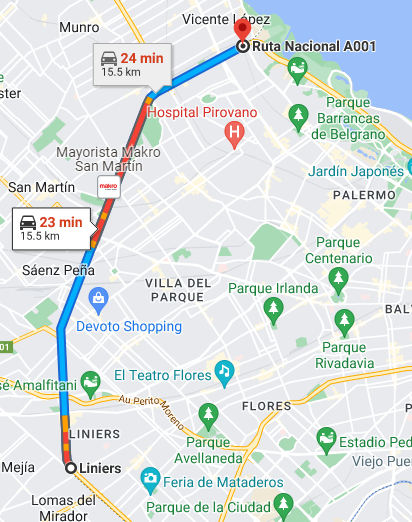
\includegraphics[width=10em]{gmaps-recorrido}
\end{figure}
\addtocounter{framenumber}{-1}
\end{frame}

\begin{frame}[fragile]

\frametitle{El lugar y el tiempo}
Buscamos simular un carril de la General Paz, mas precisamente, \href{https://www.google.com.ar/maps/dir/-34.6549026,-58.5273448/RN+A001,+Buenos+Aires/@-34.5529941,-58.5215513,13z/data=!4m9!4m8!1m0!1m5!1m1!1s0x95bcb6a69ad1fc61:0x7f1d6a8008451498!2m2!1d-58.4682776!2d-34.5357282!3e0?entry=ttu}{\textcolor{blue}{el trayecto desde Liniers hasta Lugones}} (15.5 km). 

\begin{figure}
\centering
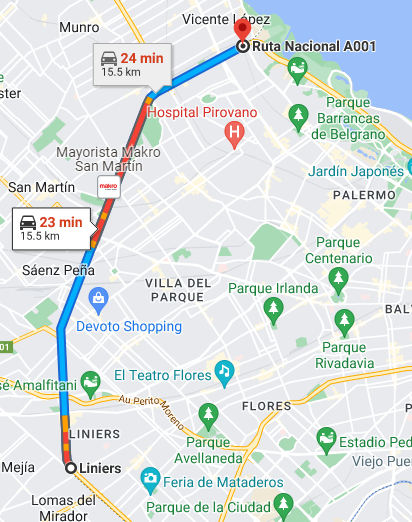
\includegraphics[width=10em]{gmaps-recorrido}
\end{figure}

Simularemos una ma\~nana de d\'ia laboral, de 5:00 AM a 10 AM.
\addtocounter{framenumber}{-1}
\end{frame}

\begin{frame}[fragile]

\frametitle{Agentes}

Llamamos agentes a los conductores y su auto como un conjunto. Estos, poseen tres caracter\'isticas:

\end{frame}

\begin{frame}[fragile]

\frametitle{Agentes}

Llamamos agentes a los conductores y su auto como un conjunto. Estos, poseen tres caracter\'isticas:

\begin{itemize}
\item $\mathcal{T}$: Headway -> Distancia en segundos que desea tener el agente con el agente que est\'a delante.
\end{itemize}
\addtocounter{framenumber}{-1}
\end{frame}
\begin{frame}[fragile]

\frametitle{Agentes}

Llamamos agentes a los conductores y su auto como un conjunto. Estos, poseen tres caracter\'isticas:

\begin{itemize}
\item $\mathcal{T}$: Headway -> Distancia en segundos que desea tener el agente con el agente que est\'a delante.
\item $v_0$: Velocidad deseada -> Velocidad a la que le gustar\'ia ir al agente en caso de no estar restringido, representada en $m/s$.
\end{itemize}
\addtocounter{framenumber}{-1}
\end{frame}

\begin{frame}[fragile]

\frametitle{Agentes}

Llamamos agentes a los conductores y su auto como un conjunto. Estos, poseen tres caracter\'isticas:

\begin{itemize}
\item $\mathcal{T}$: Headway -> Distancia en segundos que desea tener el agente con el agente que est\'a delante.
\item $v_0$: Velocidad deseada -> Velocidad a la que le gustar\'ia ir al agente en caso de no estar restringido, representada en $m/s$.
\item $l$: Longitud del veh\'iculo -> Longitud del auto del agente en metros.
\end{itemize}
\addtocounter{framenumber}{-1}
\end{frame}

\begin{frame}[fragile]

\frametitle{Reglas de interacci\'on}
\begin{itemize}
\item Cada agente tiene una posici\'on $X_t$ que se modifica en cada fracci\'on de tiempo $t$, en nuestro caso de a 1s.
\end{itemize}


\end{frame}

\begin{frame}[fragile]

\frametitle{Reglas de interacci\'on}
\begin{itemize}
\item Cada agente tiene una posici\'on $X_t$ que se modifica en cada fracci\'on de tiempo $t$, en nuestro caso de a 1s.
\item A su vez, tienen una velocidad $V_t$.
\end{itemize}
\addtocounter{framenumber}{-1}
\end{frame}

\begin{frame}[fragile]

\frametitle{Reglas de interacci\'on}
\begin{itemize}
\item Cada agente tiene una posici\'on $X_t$ que se modifica en cada fracci\'on de tiempo $t$, en nuestro caso de a 1s.
\item A su vez, tienen una velocidad $V_t$.
\end{itemize}
Ambas se modifican segun las leyes f\'isicas de movimiento:
\addtocounter{framenumber}{-1}
\end{frame}

\begin{frame}[fragile]

\frametitle{Reglas de interacci\'on}
\begin{itemize}
\item Cada agente tiene una posici\'on $X_t$ que se modifica en cada fracci\'on de tiempo $t$, en nuestro caso de a 1s.
\item A su vez, tienen una velocidad $V_t$.
\end{itemize}
Ambas se modifican segun las leyes f\'isicas de movimiento:
\begin{itemize}
\item $X_{t+1} = X_t + V_t * \Delta t$
\end{itemize}
\addtocounter{framenumber}{-1}
\end{frame}

\begin{frame}[fragile]

\frametitle{Reglas de interacci\'on}
\begin{itemize}
\item Cada agente tiene una posici\'on $X_t$ que se modifica en cada fracci\'on de tiempo $t$, en nuestro caso de a 1s.
\item A su vez, tienen una velocidad $V_t$.
\end{itemize}
Ambas se modifican segun las leyes f\'isicas de movimiento:
\begin{itemize}
\item $X_{t+1} = X_t + V_t * \Delta t$
\item $V_{t+1} = V_t + a_t * \Delta t$
\end{itemize}
\addtocounter{framenumber}{-1}
\end{frame}

\begin{frame}[fragile]

\frametitle{Reglas de interacci\'on}
\begin{itemize}
\item Cada agente tiene una posici\'on $X_t$ que se modifica en cada fracci\'on de tiempo $t$, en nuestro caso de a 1s.
\item A su vez, tienen una velocidad $V_t$.
\end{itemize}
Ambas se modifican segun las leyes f\'isicas de movimiento:
\begin{itemize}
\item $X_{t+1} = X_t + V_t * \Delta t$
\item $V_{t+1} = V_t + a_t * \Delta t$
\item $a_t = ?$ 
\end{itemize}
\addtocounter{framenumber}{-1}
\end{frame}

\begin{frame}[fragile]

\frametitle{Reglas de interacci\'on}
\begin{itemize}
\item Cada agente tiene una posici\'on $X_t$ que se modifica en cada fracci\'on de tiempo $t$, en nuestro caso de a 1s.
\item A su vez, tienen una velocidad $V_t$.
\end{itemize}
Ambas se modifican segun las leyes f\'isicas de movimiento:
\begin{itemize}
\item $X_{t+1} = X_t + V_t * \Delta t$
\item $V_{t+1} = V_t + a_t * \Delta t$
\item $a_t = ?$ 
\end{itemize}

Los agentes toman decisiones en su aceleraci\'on, pudiendo frenar, mantenerla constante, o acelerar. Para determinar como lo hacen, utilizaremos un modelo conocido, llamado Intelligent Driver Model (IDM). \supercite{1}
\addtocounter{framenumber}{-1}
\end{frame}

\begin{frame}[fragile]

\frametitle{Intelligent Driver Model}
El Intelligent Driver Model actualiza la posici\'on y velocidad como mencionamos anteriormente.

\end{frame}
\begin{frame}[fragile]

\frametitle{Intelligent Driver Model}
El Intelligent Driver Model actualiza la posici\'on y velocidad como mencionamos anteriormente. El calculo de la aceleraci\'on es el siguiente, con $\alpha$ el n\'umero de agente y $\alpha - 1$ el agente de adelante.

  \begin{equation*}
    a_t = a (1 - (\frac{v_\alpha}{v_0})^2 - (\frac{s_0 + v\mathcal{T} + (\frac{v_\alpha (v_\alpha - v_{\alpha-1})}{2\sqrt{ab}})}{x_{\alpha-1} - x_\alpha - l_{\alpha-1}})^2
  \end{equation*}
\addtocounter{framenumber}{-1}
\end{frame}

\begin{frame}[fragile]

\frametitle{Intelligent Driver Model}
El Intelligent Driver Model actualiza la posici\'on y velocidad como mencionamos anteriormente. El calculo de la aceleraci\'on es el siguiente, con $\alpha$ el n\'umero de agente y $\alpha - 1$ el agente de adelante.

  \begin{equation*}
    a_t = a (1 - (\frac{v_\alpha}{v_0})^2 - (\frac{s_0 + v\mathcal{T} + (\frac{v_\alpha (v_\alpha - v_{\alpha-1})}{2\sqrt{ab}})}{x_{\alpha-1} - x_\alpha - l_{\alpha-1}})^2
  \end{equation*}

Donde:
\begin{itemize}
\item $v_0$: La velocidad deseada del agente.
\end{itemize}
\addtocounter{framenumber}{-1}
\end{frame}

\begin{frame}[fragile]

\frametitle{Intelligent Driver Model}
El Intelligent Driver Model actualiza la posici\'on y velocidad como mencionamos anteriormente. El calculo de la aceleraci\'on es el siguiente, con $\alpha$ el n\'umero de agente y $\alpha - 1$ el agente de adelante.

  \begin{equation*}
    a_t = a (1 - (\frac{v_\alpha}{v_0})^2 - (\frac{s_0 + v\mathcal{T} + (\frac{v_\alpha (v_\alpha - v_{\alpha-1})}{2\sqrt{ab}})}{x_{\alpha-1} - x_\alpha - l_{\alpha-1}})^2
  \end{equation*}

Donde:
\begin{itemize}
\item $v_0$: La velocidad deseada del agente.
\item $s_0$: La minima distancia neta en metros (un auto no puede moverse si el de adelante esta a menos de $s_0$).
\end{itemize}
\addtocounter{framenumber}{-1}
\end{frame}

\begin{frame}[fragile]

\frametitle{Intelligent Driver Model}
El Intelligent Driver Model actualiza la posici\'on y velocidad como mencionamos anteriormente. El calculo de la aceleraci\'on es el siguiente, con $\alpha$ el n\'umero de agente y $\alpha - 1$ el agente de adelante.

  \begin{equation*}
    a_t = a (1 - (\frac{v_\alpha}{v_0})^2 - (\frac{s_0 + v\mathcal{T} + (\frac{v_\alpha (v_\alpha - v_{\alpha-1})}{2\sqrt{ab}})}{x_{\alpha-1} - x_\alpha - l_{\alpha-1}})^2
  \end{equation*}

Donde:
\begin{itemize}
\item $v_0$: La velocidad deseada del agente.
\item $s_0$: La minima distancia neta en metros (un auto no puede moverse si el de adelante esta a menos de $s_0$).
\item $\mathcal{T}$: El headway del agente.
\end{itemize}
\addtocounter{framenumber}{-1}
\end{frame}

\begin{frame}[fragile]

\frametitle{Intelligent Driver Model}
El Intelligent Driver Model actualiza la posici\'on y velocidad como mencionamos anteriormente. El calculo de la aceleraci\'on es el siguiente, con $\alpha$ el n\'umero de agente y $\alpha - 1$ el agente de adelante.

  \begin{equation*}
    a_t = a (1 - (\frac{v_\alpha}{v_0})^2 - (\frac{s_0 + v\mathcal{T} + (\frac{v_\alpha (v_\alpha - v_{\alpha-1})}{2\sqrt{ab}})}{x_{\alpha-1} - x_\alpha - l_{\alpha-1}})^2
  \end{equation*}

Donde:
\begin{itemize}
\item $v_0$: La velocidad deseada del agente.
\item $s_0$: La minima distancia neta en metros (un auto no puede moverse si el de adelante esta a menos de $s_0$).
\item $\mathcal{T}$: El headway del agente.
\item $a$: La aceleraci\'on m\'axima posible del veh\'culo en $m/s^2$.
\end{itemize}
\addtocounter{framenumber}{-1}
\end{frame}

\begin{frame}[fragile]

\frametitle{Intelligent Driver Model}
El Intelligent Driver Model actualiza la posici\'on y velocidad como mencionamos anteriormente. El calculo de la aceleraci\'on es el siguiente, con $\alpha$ el n\'umero de agente y $\alpha - 1$ el agente de adelante.

  \begin{equation*}
    a_t = a (1 - (\frac{v_\alpha}{v_0})^2 - (\frac{s_0 + v\mathcal{T} + (\frac{v_\alpha (v_\alpha - v_{\alpha-1})}{2\sqrt{ab}})}{x_{\alpha-1} - x_\alpha - l_{\alpha-1}})^2
  \end{equation*}

Donde:
\begin{itemize}
\item $v_0$: La velocidad deseada del agente.
\item $s_0$: La minima distancia neta en metros (un auto no puede moverse si el de adelante esta a menos de $s_0$).
\item $\mathcal{T}$: El headway del agente.
\item $a$: La aceleraci\'on m\'axima posible del veh\'culo en $m/s^2$.
\item $b$: La desaceleraci\'on maxima posible del veh\'iculo en $m/s^2$ (valor absoluto).
\end{itemize}
\addtocounter{framenumber}{-1}
\end{frame}

\begin{frame}[fragile]

\frametitle{Los par\'ametros seleccionados}

\begin{itemize}

\item $\mathcal{T}$: Valor obtenido de una lognormal con $\mu = 0.5$, $\sigma = 0.21$ (aproximadamente, valores entre 1 y 2.5 para cada agente).

\end{itemize}

\end{frame}

\begin{frame}[fragile]

\frametitle{Los par\'ametros seleccionados}

\begin{itemize}

\item $\mathcal{T}$: Valor obtenido de una lognormal con $\mu = 0.5$, $\sigma = 0.21$ (aproximadamente, valores entre 1 y 2.5 para cada agente).
\item $v_0$: Valores entre 65 y 105 para cada agente, correlacionados con $\mathcal{T}$

\end{itemize}
\addtocounter{framenumber}{-1}
\end{frame}

\begin{frame}[fragile]

\frametitle{Los par\'ametros seleccionados}

\begin{itemize}

\item $\mathcal{T}$: Valor obtenido de una lognormal con $\mu = 0.5$, $\sigma = 0.21$ (aproximadamente, valores entre 1 y 2.5 para cada agente).
\item $v_0$: Valores entre 65 y 105 para cada agente, correlacionados con $\mathcal{T}$
\item $l$: 4.3 metros para todos los agentes (longitud de un auto promedio).

\end{itemize}
\addtocounter{framenumber}{-1}
\end{frame}

\begin{frame}[fragile]

\frametitle{Los par\'ametros seleccionados}

\begin{itemize}

\item $\mathcal{T}$: Valor obtenido de una lognormal con $\mu = 0.5$, $\sigma = 0.21$ (aproximadamente, valores entre 1 y 2.5 para cada agente).
\item $v_0$: Valores entre 65 y 105 para cada agente, correlacionados con $\mathcal{T}$
\item $l$: 4.3 metros para todos los agentes (longitud de un auto promedio).
\item $s_0$: 5 metros.

\end{itemize}
\addtocounter{framenumber}{-1}
\end{frame}

\begin{frame}[fragile]
\frametitle{Los par\'ametros seleccionados}

\begin{itemize}

\item $\mathcal{T}$: Valor obtenido de una lognormal con $\mu = 0.5$, $\sigma = 0.21$ (aproximadamente, valores entre 1 y 2.5 para cada agente).
\item $v_0$: Valores entre 65 y 105 para cada agente, correlacionados con $\mathcal{T}$
\item $l$: 4.3 metros para todos los agentes (longitud de un auto promedio).
\item $s_0$: 5 metros.
\item $a$: 2 $m/s^2$ -> Límites físicos charlados en clase.

\end{itemize}
\addtocounter{framenumber}{-1}
\end{frame}

\begin{frame}[fragile]
\frametitle{Los par\'ametros seleccionados}

\begin{itemize}

\item $\mathcal{T}$: Valor obtenido de una lognormal con $\mu = 0.5$, $\sigma = 0.21$ (aproximadamente, valores entre 1 y 2.5 para cada agente).
\item $v_0$: Valores entre 65 y 105 para cada agente, correlacionados con $\mathcal{T}$
\item $l$: 4.3 metros para todos los agentes (longitud de un auto promedio).
\item $s_0$: 5 metros.
\item $a$: 2 $m/s^2$ -> Límites físicos charlados en clase.
\item $b$: 4 $m/s^2$ -> Límites físicos charlados en clase.

\end{itemize}
\addtocounter{framenumber}{-1}
\end{frame}

\begin{frame}[fragile]
\frametitle{Los par\'ametros seleccionados}

\begin{itemize}

\item $\mathcal{T}$: Valor obtenido de una lognormal con $\mu = 0.5$, $\sigma = 0.21$ (aproximadamente, valores entre 1 y 2.5 para cada agente).
\item $v_0$: Valores entre 65 y 105 para cada agente, correlacionados con $\mathcal{T}$
\item $l$: 4.3 metros para todos los agentes (longitud de un auto promedio).
\item $s_0$: 5 metros.
\item $a$: 2 $m/s^2$ -> Límites físicos charlados en clase.
\item $b$: 4 $m/s^2$ -> Límites físicos charlados en clase.
\item $\gamma$: Un nuevo par\'ametro que determina la proporci\'on de personas con waze o gmaps alertandolos de los radares. Simulamos con distintas proporciones: 0.2, 0.4 y 0.7.

\end{itemize}
\addtocounter{framenumber}{-1}
\end{frame}

\section{Resultados}
\addtocounter{framenumber}{-1}
\begin{frame}[fragile]
\frametitle{Cambio en los par\'ametros}

\begin{itemize}
\item Objetivo original: efecto uso de app de alerta de radares.
\end{itemize}

\end{frame}

\begin{frame}[fragile]
\frametitle{Cambio en los par\'ametros}

\begin{itemize}
\item Objetivo original: efecto uso de app de alerta de radares.
	\begin{itemize}
	\item Variabilidad de velocidades de los agentes.
	\end{itemize}
\end{itemize}
\addtocounter{framenumber}{-1}
\end{frame}

\begin{frame}[fragile]
\frametitle{Cambio en los par\'ametros}

\begin{itemize}
\item Objetivo original: efecto uso de app de alerta de radares.
	\begin{itemize}
	\item Variabilidad de velocidades de los agentes.
	\item Limitaci\'on de un solo carril.
	\end{itemize}
\end{itemize}
\addtocounter{framenumber}{-1}
\end{frame}

\begin{frame}[fragile]
\frametitle{Cambio en los par\'ametros}

\begin{itemize}
\item Objetivo original: efecto uso de app de alerta de radares.
	\begin{itemize}
	\item Variabilidad de velocidades de los agentes.
	\item Limitaci\'on de un solo carril.
	\item Animaci\'on \href{https://youtu.be/NnljPUTmnGE}{\textcolor{blue}{ac\'a.}}
	\end{itemize}
\end{itemize}
\addtocounter{framenumber}{-1}
\end{frame}

\begin{frame}[fragile]
\frametitle{Cambio en los par\'ametros}

\begin{itemize}
\item Objetivo original: efecto uso de app de alerta de radares.
	\begin{itemize}
	\item Variabilidad de velocidades de los agentes.
	\item Limitaci\'on de un solo carril.
	\item Animaci\'on \href{https://youtu.be/NnljPUTmnGE}{\textcolor{blue}{ac\'a.}}
	\end{itemize}
\item Nuevo objetivo: simular el carril r\'apido
\end{itemize}
\addtocounter{framenumber}{-1}
\end{frame}

\begin{frame}[fragile]
\frametitle{Cambio en los par\'ametros}

\begin{itemize}
\item Objetivo original: efecto uso de app de alerta de radares.
	\begin{itemize}
	\item Variabilidad de velocidades de los agentes.
	\item Limitaci\'on de un solo carril.
	\item Animaci\'on \href{https://youtu.be/NnljPUTmnGE}{\textcolor{blue}{ac\'a.}}
	\end{itemize}
\item Nuevo objetivo: simular el carril r\'apido
	\begin{itemize}
	\item $v_0$ m\'as altas (entre 75km/h y 105km/h) correlacionadas con $\mathcal{T}$.
	\end{itemize}
\end{itemize}
\addtocounter{framenumber}{-1}
\end{frame}

\begin{frame}[fragile]
\frametitle{Cambio en los par\'ametros}

\begin{itemize}
\item Objetivo original: efecto uso de app de alerta de radares.
	\begin{itemize}
	\item Variabilidad de velocidades de los agentes.
	\item Limitaci\'on de un solo carril.
	\item Animaci\'on \href{https://youtu.be/NnljPUTmnGE}{\textcolor{blue}{ac\'a.}}
	\end{itemize}
\item Nuevo objetivo: simular el carril r\'apido
	\begin{itemize}
	\item $v_0$ m\'as altas (entre 75km/h y 105km/h) correlacionadas con $\mathcal{T}$.
	\item Tambi\'en con variabilidad.
	\end{itemize}
\end{itemize}
\addtocounter{framenumber}{-1}
\end{frame}

\begin{frame}[fragile]
\frametitle{Resultados con los nuevos par\'ametros}

\centering
Distribuci\'on tiempo de viaje por densidad de tr\'afico

\begin{figure}
\centering
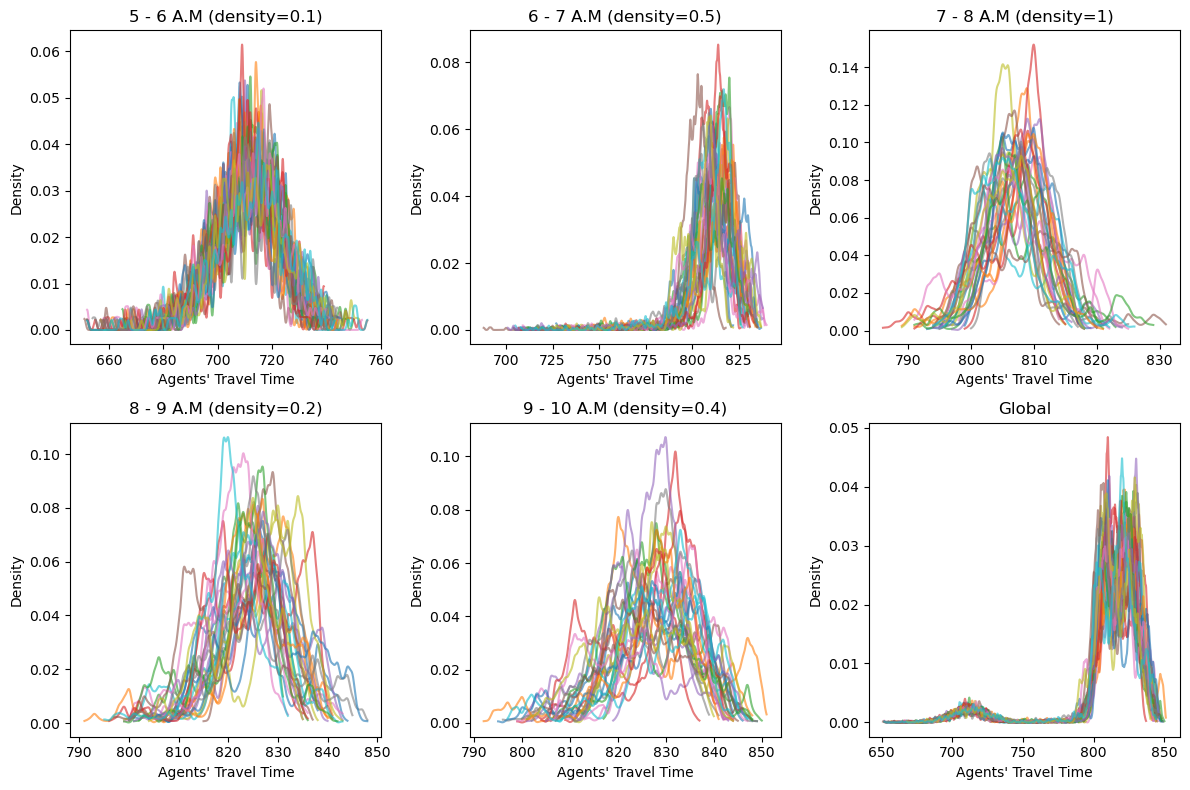
\includegraphics[width=25em]{images/travel_time_global.png}
\end{figure}


\end{frame}

\begin{frame}[fragile]
\frametitle{¿C\'omo impactan los radares en la velocidad?}
  \begin{table}
    \caption{Velocidad promedio: En rango de radar vs fuera de rango}
    \begin{tabular}{llll}
      \toprule
      Horario & En rango & Fuera de rango & Total \\
      \midrule
      5-6 AM & 20.7738 & 21.9909 & 21.8342\\
      6-7 AM & 18.1827 & 19.2592 & 19.1201\\
      7-8 AM & 18.2053 & 19.2610 & 19.1181\\
      8-9 AM & 17.8417 & 18.9392 & 18.7987\\
      9-10 AM & 17.7816 & 18.8951 & 18.7526\\
      Total & 18.1774 & 19.2730 & 19.1307\\
      \bottomrule
    \end{tabular}
  \end{table}
\end{frame}

\begin{frame}[fragile]
\frametitle{Limitaciones}

\begin{itemize}
\item Si bien ocurren cambios de velocidad, no var\'ia mucho seg\'un $\gamma$. 
\end{itemize}

\end{frame}

\begin{frame}[fragile]
\frametitle{Limitaciones}

\begin{itemize}
\item Si bien ocurren cambios de velocidad, no var\'ia mucho seg\'un $\gamma$. 
	\begin{itemize}
	\item A\'un con pocos agentes, la gran mayor\'ia disminuye la velocidad.
	\end{itemize}
\end{itemize}
\addtocounter{framenumber}{-1}
\end{frame}

\begin{frame}[fragile]
\frametitle{Limitaciones}

\begin{itemize}
\item Si bien ocurren cambios de velocidad, no var\'ia mucho seg\'un $\gamma$. 
	\begin{itemize}
	\item A\'un con pocos agentes, la gran mayor\'ia disminuye la velocidad.
	\end{itemize}
\item Choques
\end{itemize}
\addtocounter{framenumber}{-1}
\end{frame}

\begin{frame}[fragile]
\frametitle{Limitaciones}

\begin{itemize}
\item Si bien ocurren cambios de velocidad, no var\'ia mucho seg\'un $\gamma$. 
	\begin{itemize}
	\item A\'un con pocos agentes, la gran mayor\'ia disminuye la velocidad.
	\end{itemize}
\item Choques
	\begin{itemize}
	\item De 30 simulaciones, en 1 hubo choque.
	\end{itemize}
\end{itemize}
\addtocounter{framenumber}{-1}
\end{frame}

\begin{frame}[fragile]
\frametitle{Limitaciones}

\begin{itemize}
\item Si bien ocurren cambios de velocidad, no var\'ia mucho seg\'un $\gamma$. 
	\begin{itemize}
	\item A\'un con pocos agentes, la gran mayor\'ia disminuye la velocidad.
	\end{itemize}
\item Choques
	\begin{itemize}
	\item De 30 simulaciones, en 1 hubo choque.
	\item Propagaci\'on irreal.
	\end{itemize}
\end{itemize}
\addtocounter{framenumber}{-1}
\end{frame}

\begin{frame}[fragile]
\frametitle{Limitaciones}

\begin{itemize}
\item Si bien ocurren cambios de velocidad, no var\'ia mucho seg\'un $\gamma$. 
	\begin{itemize}
	\item A\'un con pocos agentes, la gran mayor\'ia disminuye la velocidad.
	\end{itemize}
\item Choques
	\begin{itemize}
	\item De 30 simulaciones, en 1 hubo choque.
	\item Propagaci\'on irreal.
	\item Animaci\'on \href{https://www.youtube.com/watch?v=Yan5BorT-o0}{\textcolor{blue}{ac\'a.}}
	\end{itemize}
\end{itemize}
\addtocounter{framenumber}{-1}
\end{frame}

\section{Conclusi\'on}
\addtocounter{framenumber}{-1}
\begin{frame}[fragile]
\frametitle{Tradeoff: Recaudaci\'on vs Seguridad}
Con el avance en el uso de apps que notifican de los radares parecer\'ia ser una variable interesante para hacedores de pol\'iticas p\'ublicas la proporci\'on de agentes que las usan y como su comportamiento cambia debido a esto.
\end{frame}

\begin{frame}[fragile]
\frametitle{Tradeoff: Recaudaci\'on vs Seguridad}
Con el avance en el uso de apps que notifican de los radares parecer\'ia ser una variable interesante para hacedores de pol\'iticas p\'ublicas la proporci\'on de agentes que las usan y como su comportamiento cambia debido a esto.

Creemos que este tipo de comportamientos puede generar:
\addtocounter{framenumber}{-1}
\end{frame}

\begin{frame}[fragile]
\frametitle{Tradeoff: Recaudaci\'on vs Seguridad}
Con el avance en el uso de apps que notifican de los radares parecer\'ia ser una variable interesante para hacedores de pol\'iticas p\'ublicas la proporci\'on de agentes que las usan y como su comportamiento cambia debido a esto.

Creemos que este tipo de comportamientos puede generar:

\begin{itemize}
\item Decisiones bruscas en los agentes.
\end{itemize}
\addtocounter{framenumber}{-1}
\end{frame}

\begin{frame}[fragile]
\frametitle{Tradeoff: Recaudaci\'on vs Seguridad}
Con el avance en el uso de apps que notifican de los radares parecer\'ia ser una variable interesante para hacedores de pol\'iticas p\'ublicas la proporci\'on de agentes que las usan y como su comportamiento cambia debido a esto.

Creemos que este tipo de comportamientos puede generar:

\begin{itemize}
\item Decisiones bruscas en los agentes.
\item Congestiones y mayores tiempos de viaje.
\end{itemize}
\addtocounter{framenumber}{-1}
\end{frame}

\begin{frame}[fragile]
\frametitle{Tradeoff: Recaudaci\'on vs Seguridad}
Con el avance en el uso de apps que notifican de los radares parecer\'ia ser una variable interesante para hacedores de pol\'iticas p\'ublicas la proporci\'on de agentes que las usan y como su comportamiento cambia debido a esto.

Creemos que este tipo de comportamientos puede generar:

\begin{itemize}
\item Decisiones bruscas en los agentes.
\item Congestiones y mayores tiempos de viaje.
\item Accidentes.
\end{itemize}
\addtocounter{framenumber}{-1}
\end{frame}

\begin{frame}[fragile]
\frametitle{Tradeoff: Recaudaci\'on vs Seguridad}
Con el avance en el uso de apps que notifican de los radares parecer\'ia ser una variable interesante para hacedores de pol\'iticas p\'ublicas la proporci\'on de agentes que las usan y como su comportamiento cambia debido a esto.

Creemos que este tipo de comportamientos puede generar:

\begin{itemize}
\item Decisiones bruscas en los agentes.
\item Congestiones y mayores tiempos de viaje.
\item Accidentes.
\end{itemize}

Vimos el cambio en las velocidades, pero no pudimos observar todas estas cosas con las limitaciones que tiene el modelo. Sin embargo, nos sirvi\'o para notar la problem\'atica y tener un punto de partida.
\addtocounter{framenumber}{-1}
\end{frame}

\begin{frame}[fragile]
\frametitle{Conclusi\'on final}

A lo largo del proyecto observamos:
\begin{itemize}
\item Distintas duraciones de viaje seg\'un densidad de tr\'afico.
\end{itemize}
\end{frame}

\begin{frame}[fragile]
\frametitle{Conclusi\'on final}

A lo largo del proyecto observamos:
\begin{itemize}
\item Distintas duraciones de viaje seg\'un densidad de tr\'afico.
\item \textit{Shockwaves} por micro-interacciones de los agentes.
\end{itemize}
\addtocounter{framenumber}{-1}
\end{frame}

\begin{frame}[fragile]
\frametitle{Conclusi\'on final}

A lo largo del proyecto observamos:
\begin{itemize}
\item Distintas duraciones de viaje seg\'un densidad de tr\'afico.
\item \textit{Shockwaves} por micro-interacciones de los agentes.
\item Variaci\'on de la velocidad promedio en base al tr\'afico.
\end{itemize}
\addtocounter{framenumber}{-1}
\end{frame}

\begin{frame}[fragile]
\frametitle{Conclusi\'on final}

A lo largo del proyecto observamos:
\begin{itemize}
\item Distintas duraciones de viaje seg\'un densidad de tr\'afico.
\item \textit{Shockwaves} por micro-interacciones de los agentes.
\item Variaci\'on de la velocidad promedio en base al tr\'afico.
\item Efecto de los radares en la velocidad de los agentes.
\end{itemize}
\addtocounter{framenumber}{-1}
\end{frame}

\begin{frame}[fragile]
\frametitle{Conclusi\'on final}

A lo largo del proyecto observamos:
\begin{itemize}
\item Distintas duraciones de viaje seg\'un densidad de tr\'afico.
\item \textit{Shockwaves} por micro-interacciones de los agentes.
\item Variaci\'on de la velocidad promedio en base al tr\'afico.
\item Efecto de los radares en la velocidad de los agentes.
\item Como podemos generar informaci\'on valiosa a partir de modelos de la realidad, que nos permiten sacar conclusiones o encontrar puntos de inter\'es, a pesar de sus limitaciones.
\end{itemize}
\addtocounter{framenumber}{-1}
\end{frame}

\begin{frame}[fragile]

\frametitle{Referencias}

\textbf{Referencias}:
\begin{itemize}
\item [{[1]}] Treiber, M., Hennecke, A., \& Helbing, D. (2000). Congested traffic states in empirical observations and microscopic simulations. Physical review E, 62(2), 1805.
\end{itemize}
 
\end{frame}
\plain{¿Preguntas?}
\end{document}
